\subsection{Photometric classification}

\myparagraph{Method}

The aim of this investigation is to analyse the affect a particular cadence has
on ones ability to photometrically classify supernova. This investigation has been carried out by the
developers of {\tt snmachine}, a DESC product that is used as a photometric
classification pipeline \cite{lochner2016photometric}.

The motivation for this work comes from the desire to identify as many \sne in order to help constrain the nature of Dark Energy.
LSST will observe many more Supernova than ever before, but at a rate that is
not feasible for all of these transients to be spectroscopically followed up and
confirmed as Type 1a or not. Thus, the ability to classify these objects photometrically will be very
important. If one can obtain a greater set of \sne, an updated Hubble
digram plot can be produced and the fundamental parameters of the cosmological
model can be tested further.

In order to conduct this analysis, a third
party software, {\tt SNANA}, has been used to generate light curves that correspond to
different cadences runs from \opsim outputs. The generated light curves are
then used as inputs in the {\tt snmachine} pipeline, an example of which is
shown below.

An interpolation is done for the between the sampled points to produce a smooth
light curves with one can then apply a wavelet decomposition to. The resulting
wavelet coefficients are then processed further to reduce dimensionality using a
principle component analysis. These principle components are then
provided as features to a random forest classifier. To ensure a controlled test,
for each cadence run a classifier is trained on 2000 light
curves only and then tested on the remaining set of light curves that are in the
corresponding dataset produced from {\tt SNANA} in relation to specific \opsim cadence
simulations. 

\myparagraph{Results}

%The results for which are shown below in Figure\ref{fig:rocs}
\begin{figure}
  \centering
  \subfigure[DDFY1]{\label{fig:ddfy1}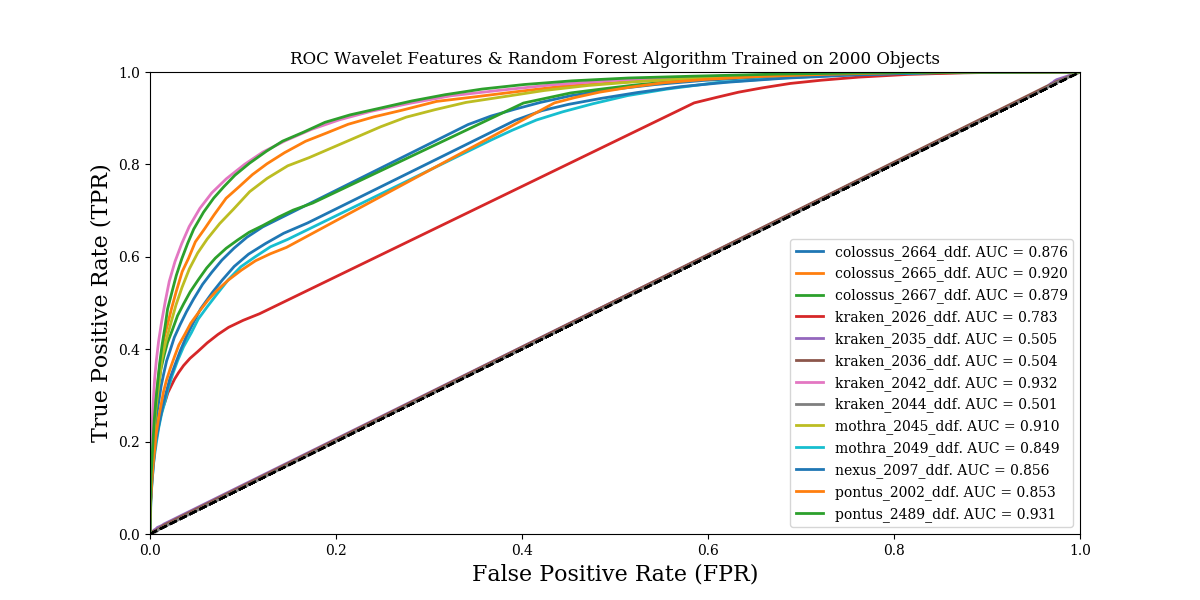
\includegraphics[width=0.8\textwidth]{classification/photometric_classification_roc_results_ddfY1.png}}
    \subfigure[DDFY10]{\label{fig:ddfy10}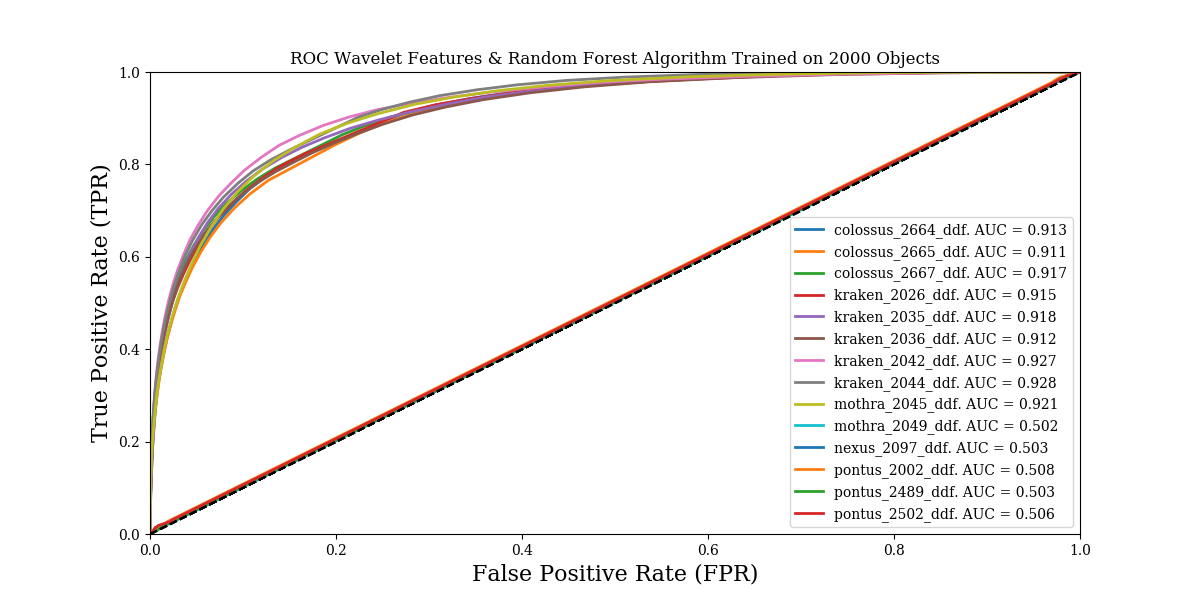
\includegraphics[width=0.8\textwidth]{classification/photometric_classification_roc_results_ddfY10.png}}
   \caption{Comparison for the DDFY1 and DDFY10 ROC curves}\label{fig:rocs}
\end{figure}

Figure \ref{fig:ddfy1}~shows the comparative classification performance between 13 cadences for the Deep
Drilling Fields of Year 1 whereas Figure \ref{fig:ddfy10}~compares the same
cadences for the Deep Drilling Fields over the entire survey.

The area under the Receiver Operating Characteristic (auROC) curves were chosen as the metric
to evaluate the performance. It was felt this single scalar would be most useful
for being able to differentiate the ability of the various cadence strategies
to perform photometric classification.


\myparagraph{Conclusion}

By interpolating the sampled light curved with Gaussian process and then applying a
wavelet decomposition to these interpolated light curves, one obtains features
that can be provided to a classifier, in this case a Random Forest algorithm.

 The performance of the interpolation is directly affected by the amount of samples one has on the light curve. More samples improves the reliability of the Gaussian processes and thus provided better features via the wave decomposition.

 Therefore it can be understood that in order to classify transients, short sampling of a light curve is important. This is particularly crucial for early classification leading to possible spectroscopic follow up.

 The results for the DDFY1 case show a significant difference in classification performance between cadences, with kraken\_2042 being most favourable. This cadences has single 30 second snaps in all bands, thus providing better sampling along the light curve. This is one of the elements that could explain the good performance, and further studies are being carried out to explore which other elements of cadence result in better classification performance.

 Further analysis was also done on Wide-Fast-Deep (WFD) cadence runs with work in progress for models trained on DDF and then tested on WFD.


